\documentclass[a4paper,12pt, english]{article}
\usepackage[top=2cm, bottom=2cm, left=2cm, right=2cm]{geometry}

\usepackage{babel}
%\usepackage{amsmath}

\usepackage{color}

\usepackage{listings}
\usepackage{url}


\usepackage{graphicx}
\usepackage{caption}
\usepackage{subcaption}

\usepackage{verbatim}

%\usepackage{caption}
%\usepackage{enumitem}

%\onehalfspacing

\begin{document}

\title{A List of Regression Models' Evaluation Metrics}
%\\ \small{\url{http://weka.sourceforge.net/doc.dev/weka/classifiers/Evaluation.html}}
\date{31 Jul 2014}
\author{By: Noureddin Sadawi}
\maketitle

\large

\begin{enumerate}

\item \textbf{\textcolor{blue}{Error-based Measures (Sensitive stats - certainty of predictions)}} \textcolor{red}{in Expose}
\begin{enumerate}

\item \textbf{Mean Absolute Error: }
      Returns the mean absolute error. %\textcolor{red}{Expose}
     

\item \textbf{Root Mean Squared Error: }
      Returns the root mean squared error. %\textcolor{red}{Expose}
                 

\item \textbf{Relative Absolute Error: }
      Returns the relative absolute error. %\textcolor{red}{Expose}
      
          
\item \textbf{Root Relative Squared Error: }
      Returns the root relative squared error if the class is numeric. %\textcolor{red}{Expose}
      
      
\begin{figure}[h]
        \centering
        \begin{subfigure}[b]{0.23\textwidth}
                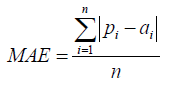
\includegraphics[width=\textwidth]{../figs/MAE}
                %\caption{A gull}
                \label{fig:mae}
        \end{subfigure} \quad %
        ~ %add desired spacing between images, e. g. ~, \quad, \qquad, \hfill etc.
          %(or a blank line to force the subfigure onto a new line)
        \begin{subfigure}[b]{0.23\textwidth}
                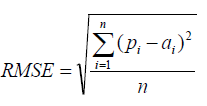
\includegraphics[width=\textwidth]{../figs/RMSE}
                %\caption{A tiger}
                \label{fig:rmse}
        \end{subfigure} 
        
         ~ %add desired spacing between images, e. g. ~, \quad, \qquad, \hfill etc.
          %(or a blank line to force the subfigure onto a new line)
        \begin{subfigure}[b]{0.23\textwidth}
                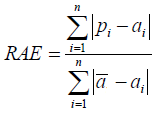
\includegraphics[width=\textwidth]{../figs/RAE}
                %\caption{A mouse}
                \label{fig:rae}
        \end{subfigure}\quad
        \begin{subfigure}[b]{0.23\textwidth}
                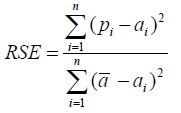
\includegraphics[width=\textwidth]{../figs/RSE}
                %\caption{A mouse}
                \label{fig:rse}
        \end{subfigure}
        
        \begin{subfigure}[b]{0.23\textwidth}
                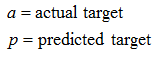
\includegraphics[width=\textwidth]{../figs/actual_predicted}
                %\caption{A mouse}
                \label{fig:ap}
        \end{subfigure}
        \caption{Metrics}\label{fig:metrics}
\end{figure}

\item \textbf{Mean Squared Error: } %\textcolor{red}{Expose}
\item \textbf{Mean Absolute Percentage Error: } %\textcolor{red}{Expose}
\item \textbf{Normalized Mean Squared Error: } %\textcolor{red}{Expose}
\item \textbf{r squared: } %\textcolor{red}{Expose}
\item \textbf{Relative Squared Error: } %\textcolor{red}{Expose}
\item \textbf{Sum Squared Error: } %\textcolor{red}{Expose}                                 
				 
\end{enumerate} 

\item \textbf{Correlation Coefficient: }
          Returns the correlation coefficient if the class is numeric.   \textcolor{red}{in Expose} 
%\newpage

\item \textbf{\textcolor{blue}{Information Criterion: }} \textcolor{red}{in Expose} 
\begin{enumerate}
\item \textbf{Akaike Information Criterion: }
\item \textbf{Bayesian Information Criterion: }          

\end{enumerate}

\item \textbf{\textcolor{blue}{Robust Error Measures: }} \textcolor{red}{in Expose}
\begin{enumerate}
\item \textbf{Alpha Trimmed Mean Square Error: }
\item \textbf{M Estimator: } 
\item \textbf{Median Squared Error: }
\end{enumerate}


\item \textbf{\textcolor{blue}{SF stats}}
\begin{enumerate}
\item \textbf{SF Prior Entropy: }
          Returns the total entropy for the null model.

\item \textbf{SF Mean Scheme Entropy: }
          Returns the entropy per instance for the scheme                  
              
\item \textbf{SF Entropy Gain:}
          Returns the total SF, which is the null model entropy minus the scheme entropy.    
          
\item \textbf{SF Mean Prior Entropy: }
          Returns the entropy per instance for the null model.       
          
\item \textbf{SF Scheme Entropy: }
          Returns the total entropy for the scheme. 

\item \textbf{SF Mean Entropy Gain: }
          Returns the SF per instance, which is the null model entropy minus the scheme entropy, per instance.         
         

\end{enumerate}

                
\item Number\_of\_training\_instances

\item Number\_of\_testing\_instances          

\item Elapsed\_Time\_training

\item Elapsed\_Time\_testing

\item UserCPU\_Time\_training

\item UserCPU\_Time\_testing
    
\item Serialized\_Model\_Size

\item Serialized\_Train\_Set\_Size

\item Serialized\_Test\_Set\_Size
	    
\end{enumerate}

%\begin{enumerate}

    %\item Number\_of\_training\_instances
    %\item Number\_of\_testing\_instances

    %\item Basic performance stats - right vs wrong - 
    %\begin{enumerate}
	  %%%  \item Number\_correct - eval.correct()
	  %%%  \item Number\_incorrect - eval.incorrect()
	  %%%  \item Number\_unclassified - eval.unclassified()
	   %%%\item Percent\_correct - eval.pctCorrect()
	   %%%\item Percent\_incorrect -  eval.pctIncorrect()
	   %%% \item Percent\_unclassified - eval.pctUnclassified()
	   %%% \item Kappa\_statistic - eval.kappa()          
    
    %\end{enumerate}

    %\item Sensitive stats - certainty of predictions 
    %\begin{enumerate}
	   %%% \item Mean\_absolute\_error - eval.meanAbsoluteError()
	   %%% \item Root\_mean\_squared\_error - eval.rootMeanSquaredError()
	   %%% \item Relative\_absolute\_error - eval.relativeAbsoluteError()
	   %%% \item Root\_relative\_squared\_error - eval.rootRelativeSquaredError()	    	                        
    
    %\end{enumerate}
    %\item SF stats  \textcolor{red}{SF stats}
    %\begin{enumerate}
	    %%% \item SF\_prior\_entropy - eval.SFPriorEntropy()
	   %%% \item SF\_scheme\_entropy - eval.SFSchemeEntropy()
	   %%% \item SF\_entropy\_gain - eval.SFEntropyGain()
	   %%% \item SF\_mean\_prior\_entropy - eval.SFMeanPriorEntropy()
	   %%% \item SF\_mean\_scheme\_entropy - eval.SFMeanSchemeEntropy()
	   %%% \item SF\_mean\_entropy\_gain - eval.SFMeanEntropyGain()
	        
   % \end{enumerate}
    %\item K\&B stats \textcolor{red}{K\&B stats}
    %\begin{enumerate}
	  %%%  \item KB\_information -  eval.KBInformation()
	  %%%  \item KB\_mean\_information - eval.KBMeanInformation()
	  %%%  \item KB\_relative\_information - eval.KBRelativeInformation()

    %\end{enumerate}
   % \item IR stats   \textcolor{red}{IR stats}
   % \begin{enumerate}
	  %%%  \item True\_positive\_rate - eval.truePositiveRate(m\_IRclass)
	    %%%\item Num\_true\_positives - eval.numTruePositives(m\_IRclass)
	  %%%  \item False\_positive\_rate - eval.falsePositiveRate(m\_IRclass)
	  %%%  \item Num\_false\_positives -  eval.numFalsePositives(m\_IRclass)
	   %%% \item True\_negative\_rate - eval.trueNegativeRate(m\_IRclass)
	  %%%  \item Num\_true\_negatives - eval.numTrueNegatives(m\_IRclass)
	  %%%  \item False\_negative\_rate - eval.falseNegativeRate(m\_IRclass)
	  %%%  \item Num\_false\_negatives - eval.numFalseNegatives(m\_IRclass)
	  %%%  \item IR\_precision - eval.precision(m\_IRclass)
	  %%%  \item IR\_recall - eval.recall(m\_IRclass)
	  %%%  \item F\_measure - eval.fMeasure(m\_IRclass)
	  %%%  \item Area\_under\_ROC -  eval.areaUnderROC(m\_IRclass)

   % \end{enumerate}
    %\item Weighted IR stats \textcolor{red}{Weighted IR stats}
    %\begin{enumerate}
	 %%%   \item Weighted\_avg\_true\_positive\_rate - eval.weightedTruePositiveRate()
	 %%%   \item Weighted\_avg\_false\_positive\_rate - eval.weightedFalsePositiveRate()
	 %%%   \item Weighted\_avg\_true\_negative\_rate - eval.weightedTrueNegativeRate()
	%%%   \item Weighted\_avg\_false\_negative\_rate - eval.weightedFalseNegativeRate()
	%%%    \item Weighted\_avg\_IR\_precision - eval.weightedPrecision()
	%%%    \item Weighted\_avg\_IR\_recall - eval.weightedRecall()
	%%%    \item Weighted\_avg\_F\_measure - eval.weightedFMeasure()
	%%%    \item Weighted\_avg\_area\_under\_ROC - eval.weightedAreaUnderROC()
  
    %\end{enumerate}
    %\item Timing stats
    %\begin{enumerate}
	    %\item Elapsed\_Time\_training
	    %\item Elapsed\_Time\_testing
	    %\item UserCPU\_Time\_training
	    %\item UserCPU\_Time\_testing
    %\end{enumerate}
    %\item sizes
    %\begin{enumerate}
	    %\item Serialized\_Model\_Size
	    %\item Serialized\_Train\_Set\_Size
	    %\item Serialized\_Test\_Set\_Size
    %\end{enumerate}
    
    %// ID/Targets/Predictions
    %if (getAttributeID() >= 0) resultNames[current++] =\item Instance\_ID
    %if (getPredTargetColumn()){
    %    resultNames[current++] =\item Targets
    %    resultNames[current++] =\item Predictions
    %}
    
%\end{enumerate}

\begin{comment}
    train.numInstances()
    eval.numInstances()
    
    
    
    
    
    
    
    // IR stats
    
    
    // Weighted IR stats
    
    
    // Timing stats
    trainTimeElapsed / 1000.0
    testTimeElapsed / 1000.0
    if(canMeasureCPUTime) {
      (trainCPUTimeElapsed/1000000.0) / 1000.0
      (testCPUTimeElapsed /1000000.0) / 1000.0
    }
    else {
      Instance.missingValue()
      Instance.missingValue()
    }
\end{comment}
\end{document}
